\label{sec:yields}
After the selections described in Section \ref{sec:event_selection}, the event yields are extracted for signal and backgrounds for each of the four periods of \Run2, for the signal and control regions.

\subsection{Four lepton channel}
The pre-fit yields for the signal and background processes for the signal region
with four leptons passing the tight selection and a photon passing the cut-based ID (SR4P\_1P),
can be seen in Table \ref{tab:Run2_SR4P_phoCR_lepCR} (Table~\ref{tab:Run2_SR4P_phoMC_lepCR})
when using the data-driven (simulation) to estimate tha fake photon background.
Alternatively, the expected yields obtained using the
working point \texttt{wp90} of the MVA ID are shown in Table~\ref{tab:Run2_SR4P_phoMC_lepCR_wp90}.

Additional tables, including also the observed number of data events, are provided
for the fake photon application region (Table \ref{tab:yields_Run2_CR4P_1F_lepCR}),
and for the fake lepton application regions (Tables \ref{tab:yields_Run2_CR3P1F_1P} and \ref{tab:yields_Run2_CR2P2F_1P}).

The yields in the triboson fiducial region are shown
in Table~\ref{tab:yield_SR4P_1P_FSRcut_Loose} for the Loose working point of the cut-based ID,
and in Table~\ref{tab:yield_SR4P_1P_FSRcut_wp90} when using the \texttt{wp80} of the MVA ID instead.

\begin{table}
  \caption{Yields from the signal region SR4P\_1P, with four leptons passing the tight selection and a photon passing the cut-based ID.
  The \nonprompt and misidentified photons are estimated with the data-driven method
  and thus only the events containing a prompt generated photon are included from the main background samples.
  }
  \label{tab:Run2_SR4P_phoCR_lepCR}
  % Note: this is from the variable mZZGloose
  \resizebox{\textwidth}{!}{%
  \begin{tabular}{lccccc}
    \toprule
    {}                            & 2016preVFP         & 2016postVFP        & 2017               & 2018               & \Run2               \\
    \midrule
    $\PZ\PZ\PGg\to4\Pl\PGg$       &  1.962 $\pm$ 0.047 &  1.714 $\pm$ 0.040 &  4.021 $\pm$ 0.100 &  5.864 $\pm$ 0.142 &  13.561 $\pm$ 0.184 \\
    $\Pg\Pg\to\PZ\PZ\to4\Pe$      &  0.031 $\pm$ 0.001 &  0.030 $\pm$ 0.001 &  0.076 $\pm$ 0.002 &  0.104 $\pm$ 0.003 &   0.240 $\pm$ 0.004 \\
    $\Pg\Pg\to\PZ\PZ\to2\Pe2\PGm$ &  0.063 $\pm$ 0.003 &  0.057 $\pm$ 0.002 &  0.069 $\pm$ 0.003 &  0.104 $\pm$ 0.004 &   0.292 $\pm$ 0.006 \\
    $\Pg\Pg\to\PZ\PZ\to4\PGm$     &  0.056 $\pm$ 0.001 &  0.046 $\pm$ 0.001 &  0.117 $\pm$ 0.003 &  0.159 $\pm$ 0.004 &   0.378 $\pm$ 0.005 \\
    $\PZ\PZ\PZ$                   &  0.007 $\pm$ 0.005 &  0.000 $\pm$ 0.000 &  0.017 $\pm$ 0.008 &  0.029 $\pm$ 0.010 &   0.053 $\pm$ 0.014 \\
    $\PQt\PAQt\PZ$+jets           &  0.011 $\pm$ 0.002 &  0.010 $\pm$ 0.002 &  0.036 $\pm$ 0.005 &  0.041 $\pm$ 0.006 &   0.098 $\pm$ 0.009 \\
    Fake photons                  &  1.357 $\pm$ 0.655 &  1.011 $\pm$ 0.509 &  1.368 $\pm$ 0.519 &  2.451 $\pm$ 0.691 &   6.187 $\pm$ 1.198 \\
    $\PW\PZ\PZ$                   &  0.000 $\pm$ 0.000 &  0.021 $\pm$ 0.012 &  0.016 $\pm$ 0.015 &  0.065 $\pm$ 0.027 &   0.102 $\pm$ 0.033 \\
    $\PW\PW\PZ$                   &  0.000 $\pm$ 0.000 &  0.040 $\pm$ 0.040 &  0.041 $\pm$ 0.041 &  0.082 $\pm$ 0.058 &   0.163 $\pm$ 0.082 \\
    \noalign{\vspace{.3ex}}\hline\noalign{\vspace{.3ex}}
    Total                         &  3.488 $\pm$ 0.656 &  2.927 $\pm$ 0.512 &  5.759 $\pm$ 0.531 &  8.900 $\pm$ 0.709 &  21.074 $\pm$ 1.215 \\
    \bottomrule
  \end{tabular}
  }
\end{table}

\begin{table}
  \caption{Yields from the signal region SR4P\_1P, with four leptons passing the tight selection and a photon passing the cut-based ID.
    The \nonprompt and misidentified photons are taken from the simulation.
  }
  \label{tab:Run2_SR4P_phoMC_lepCR}
  % Note: this is from the variable mZZGloose
  \resizebox{\textwidth}{!}{%
  \begin{tabular}{lccccc}
    \toprule
    {}                            & 2016preVFP          & 2016postVFP       & 2017               & 2018               & \Run2               \\
    \midrule
    $\PZ\PZ\PGg\to4\Pl\PGg$       &  1.962 $\pm$ 0.047 &  1.714 $\pm$ 0.040 &  4.021 $\pm$ 0.100 &  5.864 $\pm$ 0.142 &  13.561 $\pm$ 0.184 \\
    $\PQq\PAQq\to\PZ\PZ\to4\Pl$   &  0.243 $\pm$ 0.011 &  0.210 $\pm$ 0.009 &  0.610 $\pm$ 0.018 &  0.858 $\pm$ 0.025 &   1.921 $\pm$ 0.034 \\
    $\Pg\Pg\to\PZ\PZ\to4\Pe$      &  0.036 $\pm$ 0.001 &  0.035 $\pm$ 0.001 &  0.088 $\pm$ 0.002 &  0.124 $\pm$ 0.003 &   0.283 $\pm$ 0.004 \\
    $\Pg\Pg\to\PZ\PZ\to2\Pe2\PGm$ &  0.077 $\pm$ 0.003 &  0.070 $\pm$ 0.003 &  0.086 $\pm$ 0.003 &  0.127 $\pm$ 0.005 &   0.360 $\pm$ 0.007 \\
    $\Pg\Pg\to\PZ\PZ\to4\PGm$     &  0.065 $\pm$ 0.001 &  0.054 $\pm$ 0.001 &  0.139 $\pm$ 0.003 &  0.192 $\pm$ 0.005 &   0.449 $\pm$ 0.006 \\
    $\PZ\PZ\PZ$                   &  0.007 $\pm$ 0.005 &  0.003 $\pm$ 0.003 &  0.021 $\pm$ 0.009 &  0.050 $\pm$ 0.014 &   0.082 $\pm$ 0.017 \\
    $\PW\PZ\PZ$                   &  0.008 $\pm$ 0.008 &  0.028 $\pm$ 0.014 &  0.038 $\pm$ 0.020 &  0.088 $\pm$ 0.031 &   0.163 $\pm$ 0.041 \\
    $\PQt\PAQt\PZ$+jets           &  0.012 $\pm$ 0.003 &  0.011 $\pm$ 0.002 &  0.048 $\pm$ 0.006 &  0.054 $\pm$ 0.007 &   0.124 $\pm$ 0.010 \\
    Fake leptons                  &  0.047 $\pm$ 0.066 &  0.000 $\pm$ 0.000 &  0.089 $\pm$ 0.119 &  0.117 $\pm$ 0.091 &   0.253 $\pm$ 0.164 \\
    $\PW\PW\PZ$                   &  0.000 $\pm$ 0.000 &  0.040 $\pm$ 0.040 &  0.041 $\pm$ 0.041 &  0.082 $\pm$ 0.058 &   0.163 $\pm$ 0.082 \\
    Total                         &  2.458 $\pm$ 0.082 &  2.164 $\pm$ 0.059 &  5.181 $\pm$ 0.164 &  7.557 $\pm$ 0.183 &  17.360 $\pm$ 0.266 \\
    \noalign{\vspace{.3ex}}\hline\noalign{\vspace{.3ex}}
    Total                         &  3.488 $\pm$ 0.656 &  2.927 $\pm$ 0.512 &  5.759 $\pm$ 0.531 &  8.900 $\pm$ 0.709 &  21.074 $\pm$ 1.215 \\
    \bottomrule
  \end{tabular}
  }
\end{table}

\begin{table}
  \caption{Yields from the signal region SR4P\_1P, with four leptons passing the tight selection
  and a photon passing the \texttt{wp90} of the MVA based ID.
  The \nonprompt and misidentified photons are taken from the simulation.
  }
  \label{tab:Run2_SR4P_phoMC_lepCR_wp90}
  % Note: this is from the variable mZZGloose
  \resizebox{\textwidth}{!}{%
  \begin{tabular}{lccccc}
    \toprule
    {}                            & 2016preVFP          & 2016postVFP       & 2017               & 2018               & \Run2               \\
    \midrule
    $\PZ\PZ\PGg\to4\Pl\PGg$       &  2.026 $\pm$ 0.047 &  1.781 $\pm$ 0.041 &  4.294 $\pm$ 0.103 &  6.126 $\pm$ 0.143 & 14.227 $\pm$ 0.187 \\
    $\PQq\PAQq\to\PZ\PZ\to4\Pl$   &  0.192 $\pm$ 0.009 &  0.158 $\pm$ 0.008 &  0.452 $\pm$ 0.015 &  0.652 $\pm$ 0.022 &  1.453 $\pm$ 0.029 \\
    $\Pg\Pg\to\PZ\PZ\to4\Pe$      &  0.036 $\pm$ 0.001 &  0.034 $\pm$ 0.001 &  0.090 $\pm$ 0.002 &  0.120 $\pm$ 0.003 &  0.280 $\pm$ 0.004 \\
    $\Pg\Pg\to\PZ\PZ\to2\Pe2\PGm$ &  0.076 $\pm$ 0.003 &  0.068 $\pm$ 0.003 &  0.086 $\pm$ 0.003 &  0.131 $\pm$ 0.005 &  0.361 $\pm$ 0.007 \\
    $\Pg\Pg\to\PZ\PZ\to4\PGm$     &  0.066 $\pm$ 0.001 &  0.053 $\pm$ 0.001 &  0.141 $\pm$ 0.003 &  0.189 $\pm$ 0.004 &  0.449 $\pm$ 0.006 \\
    $\PZ\PZ\PZ$                   &  0.010 $\pm$ 0.006 &  0.003 $\pm$ 0.003 &  0.023 $\pm$ 0.009 &  0.040 $\pm$ 0.012 &  0.076 $\pm$ 0.016 \\
    $\PQt\PAQt\PZ$+jets           &  0.014 $\pm$ 0.003 &  0.012 $\pm$ 0.002 &  0.045 $\pm$ 0.006 &  0.057 $\pm$ 0.007 &  0.129 $\pm$ 0.010 \\
    Fake leptons                  &  0.045 $\pm$ 0.066 &  0.103 $\pm$ 0.117 &  0.107 $\pm$ 0.118 &  0.022 $\pm$ 0.081 &  0.276 $\pm$ 0.196 \\
    $\PW\PZ\PZ$                   &  0.000 $\pm$ 0.000 &  0.020 $\pm$ 0.012 &  0.063 $\pm$ 0.022 &  0.076 $\pm$ 0.029 &  0.159 $\pm$ 0.038 \\
    $\PW\PW\PZ$                   &  0.000 $\pm$ 0.000 &  0.000 $\pm$ 0.000 &  0.040 $\pm$ 0.040 &  0.080 $\pm$ 0.057 &  0.121 $\pm$ 0.070 \\
    \noalign{\vspace{.3ex}}\hline\noalign{\vspace{.3ex}}
    Total                         &  2.464 $\pm$ 0.082 &  2.233 $\pm$ 0.124 &  5.342 $\pm$ 0.165 &  7.493 $\pm$ 0.178 & 17.532 $\pm$ 0.285 \\
    \bottomrule
  \end{tabular}
  }
\end{table}

\begin{table}
\caption{Yields from the fake photon application region CR4P\_1F, with four leptons passing the tight selection and a photon passing the VeryLoose ID but failing the cut-based ID Loose.}
\label{tab:yields_Run2_CR4P_1F_lepCR}
\resizebox{\textwidth}{!}{%
  \begin{tabular}{lccccc}
    \toprule
    {}                            & 2016preVFP         & 2016postVFP        & 2017               & 2018                & \Run2               \\
    \midrule
    $\PZ\PZ\PGg\to4\Pl\PGg$       &  0.302 $\pm$ 0.019 &  0.294 $\pm$ 0.017 &  0.837 $\pm$ 0.047 &   1.191 $\pm$ 0.064 &   2.623 $\pm$ 0.083 \\
    $\PQq\PAQq\to\PZ\PZ\to4\Pl$   &  2.400 $\pm$ 0.033 &  2.283 $\pm$ 0.030 &  6.428 $\pm$ 0.058 &   9.507 $\pm$ 0.084 &  20.617 $\pm$ 0.111 \\
    $\Pg\Pg\to\PZ\PZ\to4\Pe$      &  0.060 $\pm$ 0.001 &  0.059 $\pm$ 0.001 &  0.168 $\pm$ 0.003 &   0.258 $\pm$ 0.005 &   0.546 $\pm$ 0.006 \\
    $\Pg\Pg\to\PZ\PZ\to2\Pe2\PGm$ &  0.157 $\pm$ 0.004 &  0.158 $\pm$ 0.004 &  0.224 $\pm$ 0.005 &   0.322 $\pm$ 0.008 &   0.860 $\pm$ 0.011 \\
    $\Pg\Pg\to\PZ\PZ\to4\PGm$     &  0.107 $\pm$ 0.002 &  0.092 $\pm$ 0.002 &  0.253 $\pm$ 0.004 &   0.385 $\pm$ 0.006 &   0.837 $\pm$ 0.008 \\
    $\PZ\PZ\PZ$                   &  0.039 $\pm$ 0.011 &  0.025 $\pm$ 0.011 &  0.067 $\pm$ 0.016 &   0.069 $\pm$ 0.019 &   0.200 $\pm$ 0.030 \\
    $\PW\PZ\PZ$                   &  0.064 $\pm$ 0.022 &  0.071 $\pm$ 0.023 &  0.120 $\pm$ 0.034 &   0.120 $\pm$ 0.038 &   0.376 $\pm$ 0.060 \\
    $\PW\PW\PZ$                   &  0.048 $\pm$ 0.048 &  0.046 $\pm$ 0.046 &  0.000 $\pm$ 0.000 &   0.036 $\pm$ 0.036 &   0.131 $\pm$ 0.076 \\
    $\PQt\PAQt\PZ$+jets           &  0.056 $\pm$ 0.006 &  0.050 $\pm$ 0.005 &  0.171 $\pm$ 0.011 &   0.253 $\pm$ 0.015 &   0.530 $\pm$ 0.020 \\
    Fake leptons                  &  0.030 $\pm$ 0.052 &  0.051 $\pm$ 0.047 &  0.059 $\pm$ 0.092 &   0.050 $\pm$ 0.095 &   0.191 $\pm$ 0.149 \\
    \noalign{\vspace{.3ex}}\hline\noalign{\vspace{.3ex}}
    Total                         &  3.263 $\pm$ 0.084 &  3.130 $\pm$ 0.078 &  8.327 $\pm$ 0.124 &  12.191 $\pm$ 0.154 &  26.911 $\pm$ 0.229 \\
    Data                          &  5                 &  4                 &  7                 &  13                 &  29                 \\
    \bottomrule
  \end{tabular}
  }
\end{table}

\begin{table}
\caption{Yields in CR3P1F\_1P, one of the fake lepton application regions, with three leptons passing the tight selection, one passing only a loose selection, and a photon passing the cut-based ID.}
\label{tab:yields_Run2_CR3P1F_1P}
\resizebox{\textwidth}{!}{%
  \begin{tabular}{lccccc}
  \toprule
  {}                            & 2016preVFP          & 2016postVFP       & 2017               & 2018               & \Run2              \\
  \midrule
  $\PZ\PZ\PGg\to4\Pl\PGg$       &  0.143 $\pm$ 0.013 &  0.139 $\pm$ 0.011 &  0.390 $\pm$ 0.031 &  0.506 $\pm$ 0.041 &  1.178 $\pm$ 0.055 \\
  $\PW\PZ\PGg\to3\Pl\PGnl\PGg$  &  0.213 $\pm$ 0.011 &  0.191 $\pm$ 0.008 &  0.415 $\pm$ 0.020 &  0.711 $\pm$ 0.030 &  1.530 $\pm$ 0.039 \\
  $\PZ\PGg\to\Pl\Pl\PGg$        &  0.750 $\pm$ 0.285 &  0.000 $\pm$ 0.000 &  0.463 $\pm$ 0.388 &  0.492 $\pm$ 0.447 &  1.705 $\pm$ 0.657 \\
  $\PQq\PAQq\to\PZ\PZ\to4\Pl$   &  0.103 $\pm$ 0.007 &  0.085 $\pm$ 0.006 &  0.235 $\pm$ 0.011 &  0.328 $\pm$ 0.016 &  0.751 $\pm$ 0.021 \\
  $\Pg\Pg\to\PZ\PZ\to4\Pe$      &  0.011 $\pm$ 0.001 &  0.008 $\pm$ 0.000 &  0.022 $\pm$ 0.001 &  0.037 $\pm$ 0.002 &  0.078 $\pm$ 0.002 \\
  $\Pg\Pg\to\PZ\PZ\to2\Pe2\PGm$ &  0.012 $\pm$ 0.001 &  0.012 $\pm$ 0.001 &  0.016 $\pm$ 0.001 &  0.022 $\pm$ 0.002 &  0.062 $\pm$ 0.003 \\
  $\Pg\Pg\to\PZ\PZ\to4\PGm$     &  0.003 $\pm$ 0.000 &  0.003 $\pm$ 0.000 &  0.007 $\pm$ 0.001 &  0.008 $\pm$ 0.001 &  0.020 $\pm$ 0.001 \\
  $\PW\PZ\to3\Pl\PGn$           &  0.047 $\pm$ 0.027 &  0.035 $\pm$ 0.027 &  0.135 $\pm$ 0.087 &  1.101 $\pm$ 0.319 &  1.317 $\pm$ 0.333 \\
  $\PZ\PZ\PZ$                   &  0.003 $\pm$ 0.003 &  0.000 $\pm$ 0.000 &  0.010 $\pm$ 0.006 &  0.007 $\pm$ 0.005 &  0.020 $\pm$ 0.008 \\
  $\PW\PZ\PZ$                   &  0.009 $\pm$ 0.009 &  0.000 $\pm$ 0.000 &  0.001 $\pm$ 0.012 &  0.012 $\pm$ 0.012 &  0.022 $\pm$ 0.019 \\
  $\PQt\PAQt\PZ$+jets           &  0.043 $\pm$ 0.005 &  0.039 $\pm$ 0.004 &  0.068 $\pm$ 0.007 &  0.114 $\pm$ 0.010 &  0.263 $\pm$ 0.014 \\
  Drell-Yan + jets              &  0.000 $\pm$ 0.000 &  0.000 $\pm$ 0.000 &  0.000 $\pm$ 0.000 &  0.680 $\pm$ 3.520 &  0.680 $\pm$ 3.520 \\
  \noalign{\vspace{.3ex}}\hline\noalign{\vspace{.3ex}}
  Total                         &  1.337 $\pm$ 0.287 &  0.512 $\pm$ 0.031 &  1.760 $\pm$ 0.399 &  4.017 $\pm$ 3.563 &  7.625 $\pm$ 3.597 \\
  Data                          &  1.000 $\pm$ 1.000 &  0.000 $\pm$ 0.000 &  2.000 $\pm$ 1.414 &  5.000 $\pm$ 2.236 &  8.000 $\pm$ 2.828 \\
  \bottomrule
  \end{tabular}
  }
\end{table}

\begin{table}
\caption{Yields in CR2P2F\_1P, one of the fake lepton application regions, with two leptons passing the tight selection, two passing only a loose selection, and a photon passing the cut-based ID.}
\label{tab:yields_Run2_CR2P2F_1P}
\resizebox{\textwidth}{!}{%
  \begin{tabular}{lccccc}
    \toprule
    {} & 2016preVFP & 2016postVFP & 2017 & 2018 & Run2 \\
    \midrule
    $\PZ\PZ\PGg\to4\Pl\PGg$      &   0.009 $\pm$ 0.004 &  0.005 $\pm$ 0.002 &   0.006 $\pm$ 0.004 &    0.034 $\pm$ 0.010 &    0.054 $\pm$ 0.012 \\
    $\PW\PZ\PGg\to3\Pl\PGnl\PGg$ &   0.023 $\pm$ 0.003 &  0.020 $\pm$ 0.003 &   0.034 $\pm$ 0.006 &    0.053 $\pm$ 0.008 &    0.130 $\pm$ 0.011 \\
    Drell-Yan + jets             &   6.231 $\pm$ 3.599 &  1.855 $\pm$ 1.855 &  15.810 $\pm$ 5.603 &  37.763 $\pm$ 15.469 &  61.659 $\pm$ 16.943 \\
    $\PZ\PGg\to\Pl\Pl\PGg$       &   6.600 $\pm$ 0.799 &  0.000 $\pm$ 0.000 &  13.784 $\pm$ 1.461 &   22.222 $\pm$ 2.340 &   42.606 $\pm$ 2.872 \\
    $\PQq\PAQq\to\PZ\PZ\to4\Pl$  &   0.009 $\pm$ 0.002 &  0.007 $\pm$ 0.002 &   0.015 $\pm$ 0.003 &    0.023 $\pm$ 0.004 &    0.054 $\pm$ 0.006 \\
    $\PW\PZ\to3\Pl\PGnl$         &   0.002 $\pm$ 0.022 &  0.027 $\pm$ 0.019 &   0.123 $\pm$ 0.075 &    0.151 $\pm$ 0.136 &    0.302 $\pm$ 0.158 \\
    $\PQt\PAQt\PZ$+jets          &   0.023 $\pm$ 0.004 &  0.020 $\pm$ 0.003 &   0.035 $\pm$ 0.005 &    0.055 $\pm$ 0.007 &    0.133 $\pm$ 0.010 \\
    $\PQt\PZ\PQq$                &   0.005 $\pm$ 0.008 &  0.001 $\pm$ 0.006 &   0.018 $\pm$ 0.009 &    0.024 $\pm$ 0.013 &    0.048 $\pm$ 0.019 \\
    $\PQt\PW$                    &   0.057 $\pm$ 0.057 &  0.000 $\pm$ 0.000 &   0.088 $\pm$ 0.099 &    0.000 $\pm$ 0.000 &    0.144 $\pm$ 0.114 \\
    \noalign{\vspace{.3ex}}\hline\noalign{\vspace{.3ex}}
    Total                        &   6.616 $\pm$ 0.789 & 11.123 $\pm$ 6.842 & 28.359 $\pm$ 10.849 &  50.717 $\pm$ 14.889 &  96.814 $\pm$ 19.667 \\
    Data                         &  17                 &  9                 & 23                  &  28                  &  77                  \\
    \bottomrule
  \end{tabular}
  }
\end{table}

\begin{table}
  \caption{Yields in the fiducial triboson region of the four lepton channel, using the cut-based ID selection for the photon.}
  \label{tab:yield_SR4P_1P_FSRcut_Loose}
  \resizebox{\textwidth}{!}{%
  \begin{tabular}{lrrrrr}
    \toprule
    {}                           & 2016preVFP         & 2016postVFP        & 2017               & 2018               & \Run2              \\
    \midrule
    $\PZ\PZ\PGg\to4\Pl\PGg$      &  0.841 $\pm$ 0.031 &  0.728 $\pm$ 0.026 &  1.761 $\pm$ 0.066 &  2.485 $\pm$ 0.093 &  5.815 $\pm$ 0.121 \\
    $\PQq\PAQq\to\PZ\PZ\to4\Pl$  &  0.197 $\pm$ 0.010 &  0.167 $\pm$ 0.008 &  0.504 $\pm$ 0.016 &  0.701 $\pm$ 0.023 &  1.569 $\pm$ 0.031 \\
    Fake leptons                 &  0.064 $\pm$ 0.066 &  0.000 $\pm$ 0.000 &  0.106 $\pm$ 0.115 &  0.102 $\pm$ 0.086 &  0.272 $\pm$ 0.157 \\
    $\Pg\Pg\to\PZ\PZ\to4\PGm$    &  0.009 $\pm$ 0.001 &  0.010 $\pm$ 0.000 &  0.024 $\pm$ 0.001 &  0.036 $\pm$ 0.002 &  0.079 $\pm$ 0.002 \\
    $\Pg\Pg\to\PZ\PZ\to2\Pe2\PGm$&  0.021 $\pm$ 0.002 &  0.017 $\pm$ 0.001 &  0.023 $\pm$ 0.002 &  0.032 $\pm$ 0.002 &  0.094 $\pm$ 0.004 \\
    $\Pg\Pg\to\PZ\PZ\to4\Pe$     &  0.020 $\pm$ 0.001 &  0.016 $\pm$ 0.001 &  0.042 $\pm$ 0.002 &  0.060 $\pm$ 0.003 &  0.137 $\pm$ 0.003 \\
    $\PZ\PZ\PZ$                  &  0.004 $\pm$ 0.004 &  0.003 $\pm$ 0.003 &  0.014 $\pm$ 0.007 &  0.032 $\pm$ 0.011 &  0.052 $\pm$ 0.014 \\
    $\PW\PZ\PZ$                  &  0.000 $\pm$ 0.000 &  0.014 $\pm$ 0.010 &  0.023 $\pm$ 0.017 &  0.068 $\pm$ 0.028 &  0.106 $\pm$ 0.034 \\
    $\PQt\PAQt\PZ$+jets          &  0.005 $\pm$ 0.002 &  0.004 $\pm$ 0.001 &  0.022 $\pm$ 0.004 &  0.023 $\pm$ 0.005 &  0.055 $\pm$ 0.006 \\
    \noalign{\vspace{.3ex}}\hline\noalign{\vspace{.3ex}}
    Total                        &  1.160 $\pm$ 0.073 &  0.959 $\pm$ 0.030 &  2.520 $\pm$ 0.135 &  3.539 $\pm$ 0.132 &  8.178 $\pm$ 0.205 \\
    \bottomrule
  \end{tabular}
  }
\end{table}

\begin{table}
  \caption{Yields in the fiducial triboson region of the four lepton channel, using the \texttt{wp90} of the MVA ID selection for the photon.}
  \label{tab:yield_SR4P_1P_FSRcut_wp90}
  \resizebox{\textwidth}{!}{%
  \begin{tabular}{lrrrrr}
    \toprule
    {}                            & 2016preVFP         & 2016postVFP        & 2017               & 2018               & \Run2              \\
    \midrule
    $\PZ\PZ\PGg\to4\Pl\PGg$       &  0.804 $\pm$ 0.030 &  0.694 $\pm$ 0.025 &  1.703 $\pm$ 0.065 &  2.374 $\pm$ 0.089 &  5.576 $\pm$ 0.117 \\
    $\PQq\PAQq\to\PZ\PZ\to4\Pl$   &  0.088 $\pm$ 0.006 &  0.066 $\pm$ 0.005 &  0.209 $\pm$ 0.010 &  0.292 $\pm$ 0.014 &  0.656 $\pm$ 0.019 \\
    $\Pg\Pg\to\PZ\PZ\to4\Pe$      &  0.007 $\pm$ 0.000 &  0.007 $\pm$ 0.000 &  0.017 $\pm$ 0.001 &  0.025 $\pm$ 0.001 &  0.057 $\pm$ 0.002 \\
    $\Pg\Pg\to\PZ\PZ\to2\Pe2\PGm$ &  0.011 $\pm$ 0.001 &  0.010 $\pm$ 0.001 &  0.016 $\pm$ 0.001 &  0.024 $\pm$ 0.002 &  0.061 $\pm$ 0.003 \\
    $\Pg\Pg\to\PZ\PZ\to4\PGm$     &  0.014 $\pm$ 0.001 &  0.012 $\pm$ 0.001 &  0.031 $\pm$ 0.001 &  0.043 $\pm$ 0.002 &  0.100 $\pm$ 0.003 \\
    $\PZ\PZ\PZ$                   &  0.003 $\pm$ 0.003 &  0.003 $\pm$ 0.003 &  0.010 $\pm$ 0.006 &  0.024 $\pm$ 0.009 &  0.041 $\pm$ 0.012 \\
    $\PQt\PAQt\PZ$+jets           &  0.006 $\pm$ 0.002 &  0.005 $\pm$ 0.002 &  0.019 $\pm$ 0.003 &  0.016 $\pm$ 0.004 &  0.047 $\pm$ 0.006 \\
    Fake leptons                  &  0.063 $\pm$ 0.066 &  0.000 $\pm$ 0.000 &  0.109 $\pm$ 0.115 &  0.055 $\pm$ 0.078 &  0.227 $\pm$ 0.153 \\
    $\PW\PZ\PZ$                   &  0.000 $\pm$ 0.000 &  0.007 $\pm$ 0.007 &  0.039 $\pm$ 0.018 &  0.044 $\pm$ 0.022 &  0.090 $\pm$ 0.029 \\
    \noalign{\vspace{.3ex}}\hline\noalign{\vspace{.3ex}}
    Total                         &  0.997 $\pm$ 0.072 &  0.805 $\pm$ 0.027 &  2.153 $\pm$ 0.134 &  2.898 $\pm$ 0.122 &  6.853 $\pm$ 0.197 \\
    \bottomrule
  \end{tabular}
  }
\end{table}


\begin{figure}
\subfigure [2016preVFP ] {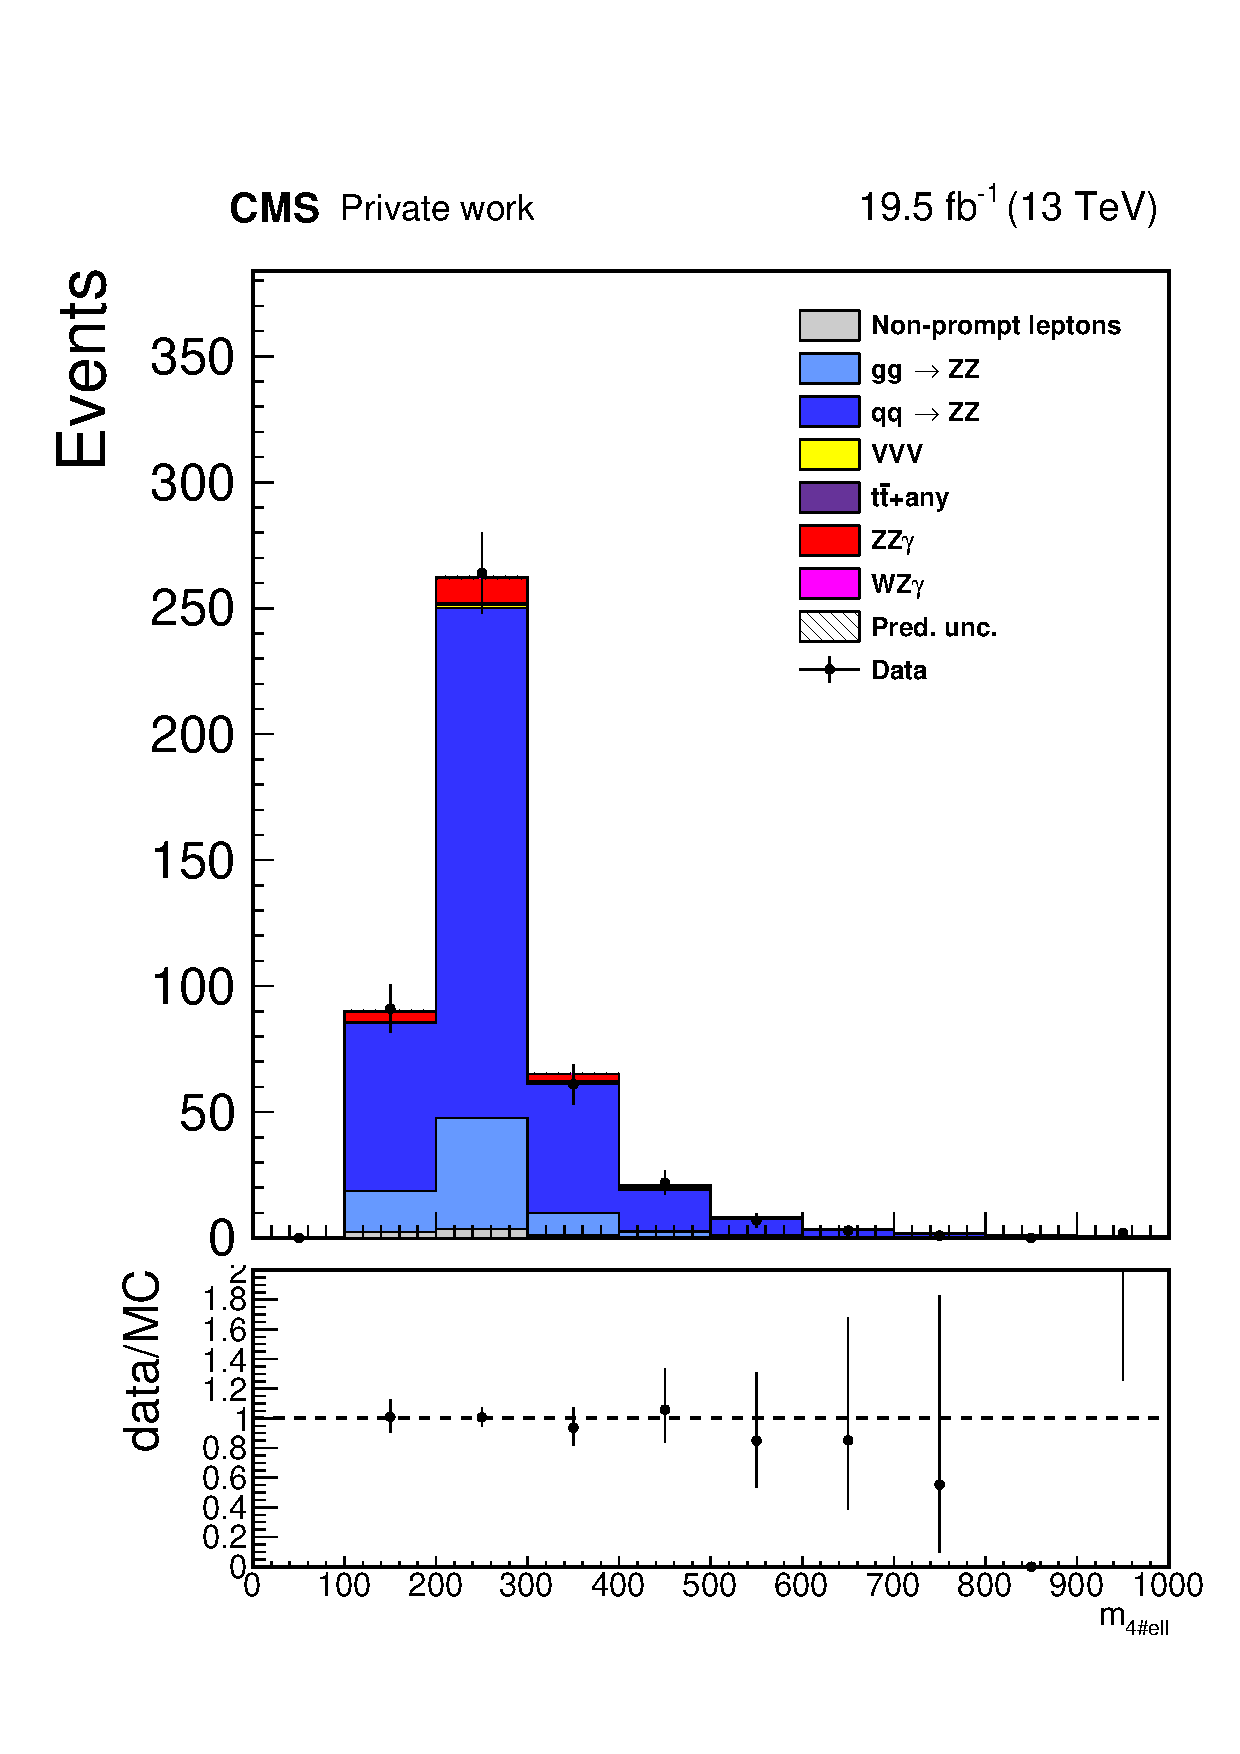
\includegraphics[width=.25\textwidth]{Figures/VVGammaAnalyzer/2016preVFP/lepCR/SR4P/ZZ_mass_pow.pdf}}%
\subfigure [2016postVFP] {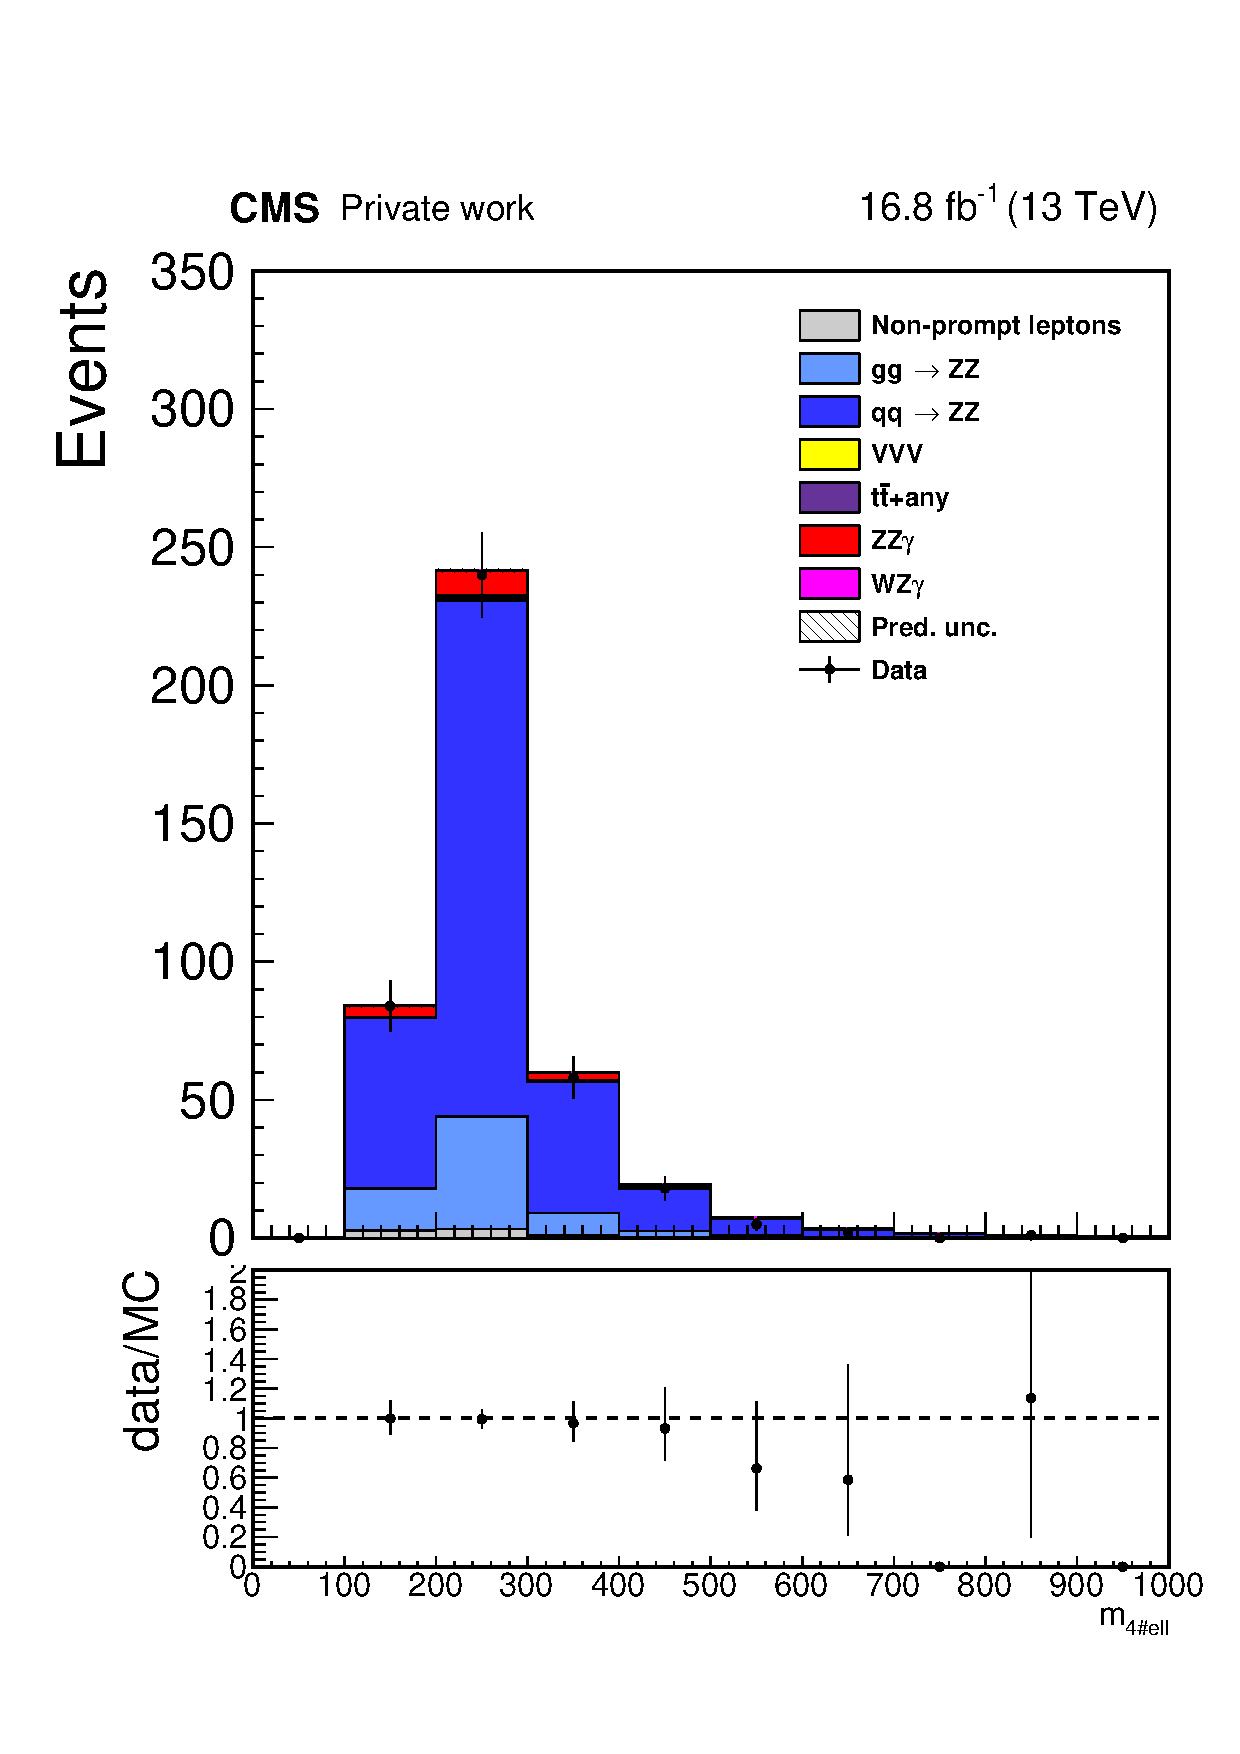
\includegraphics[width=.25\textwidth]{Figures/VVGammaAnalyzer/2016postVFP/lepCR/SR4P/ZZ_mass_pow.pdf}}%
\subfigure [2017       ] {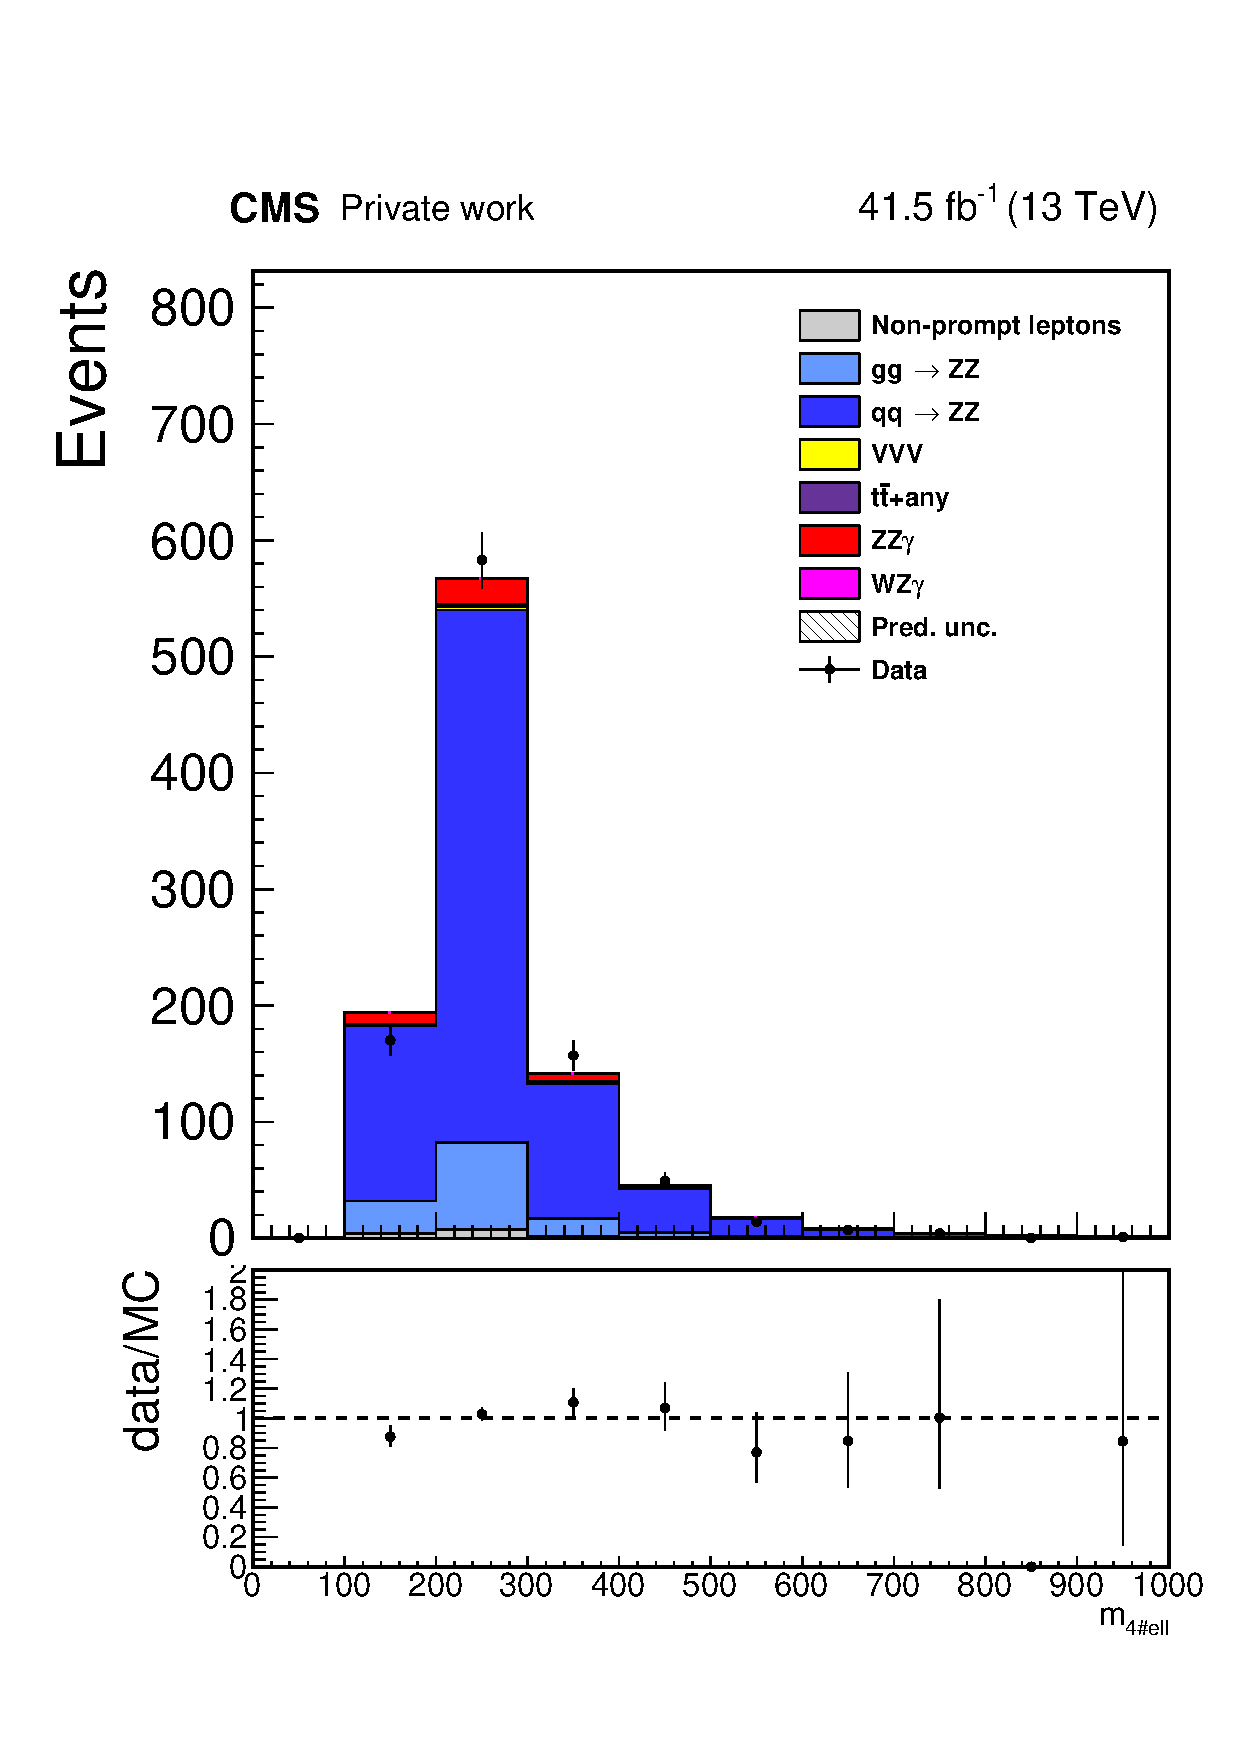
\includegraphics[width=.25\textwidth]{Figures/VVGammaAnalyzer/2017/lepCR/SR4P/ZZ_mass_pow.pdf}}%
\subfigure [2018       ] {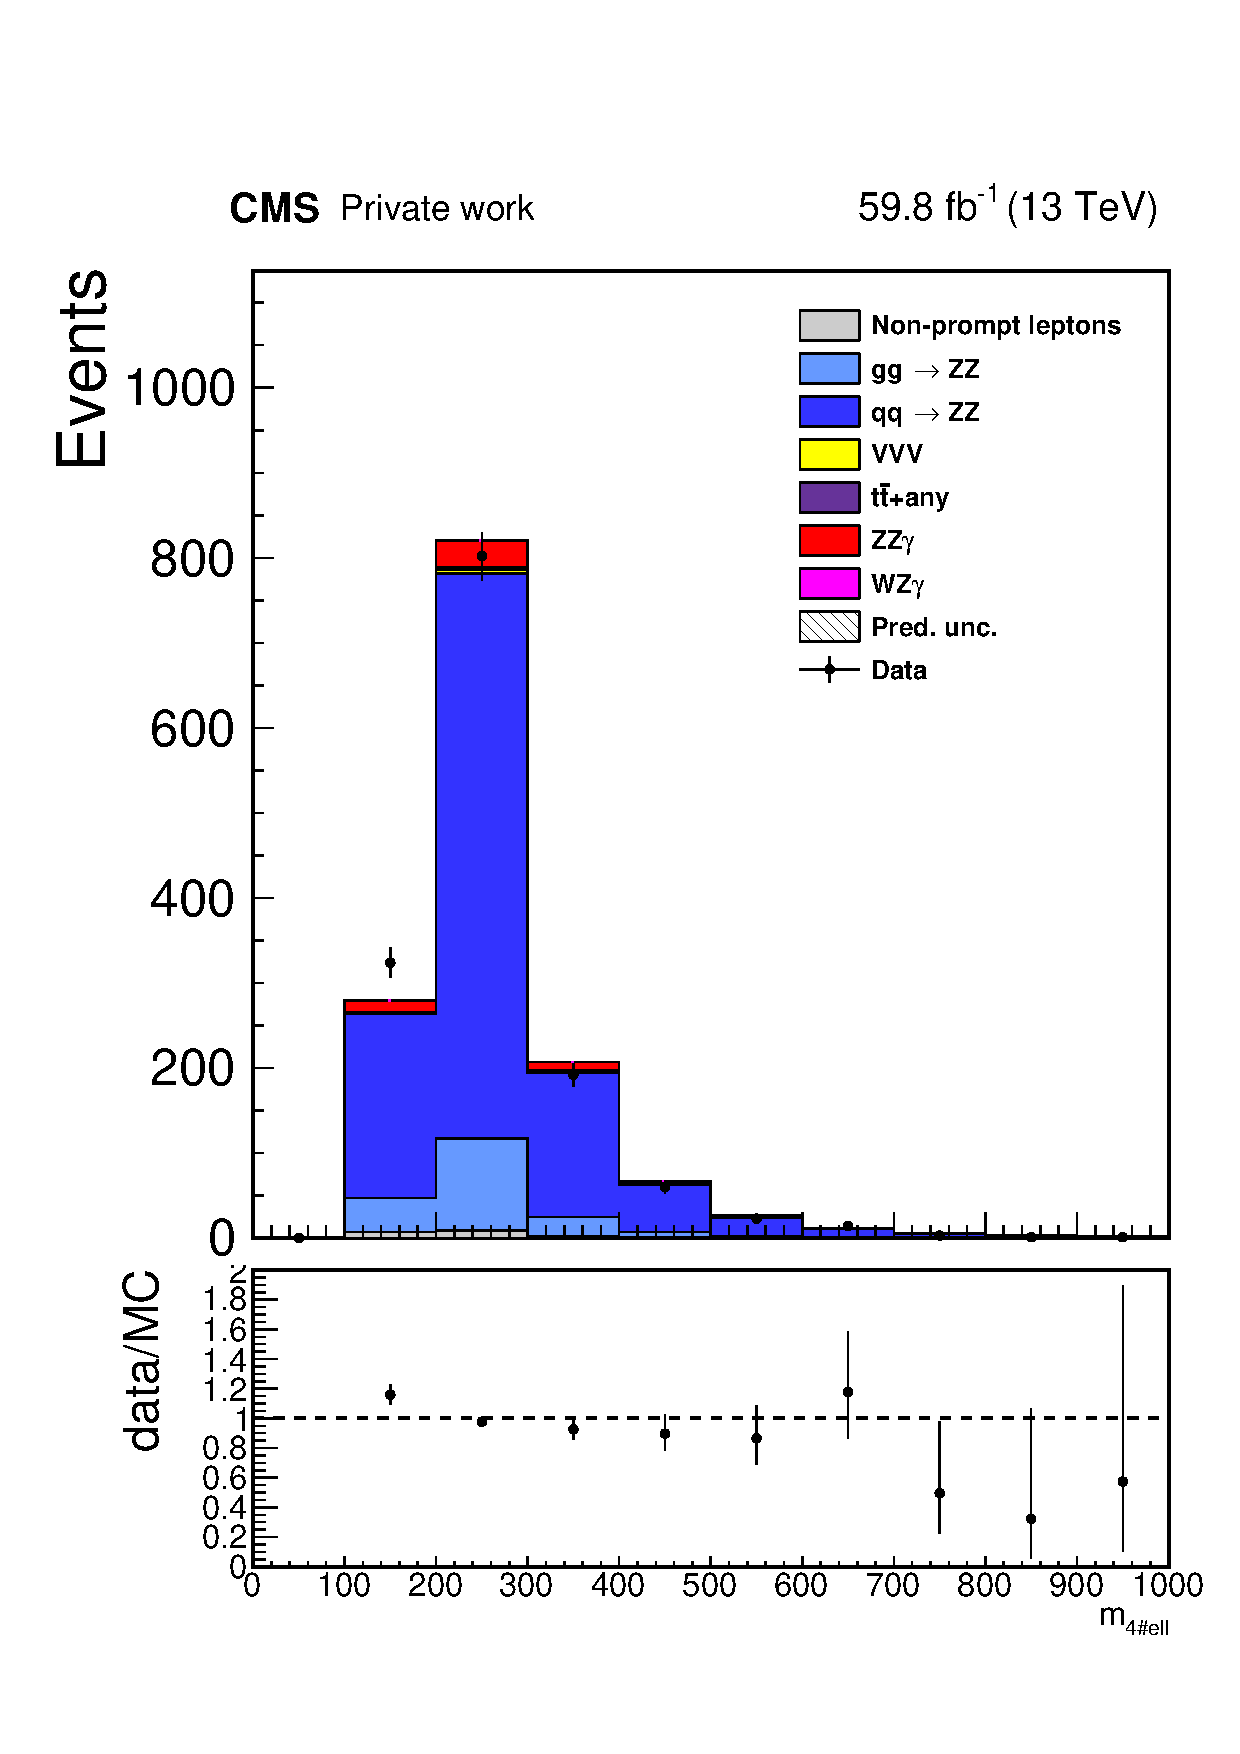
\includegraphics[width=.25\textwidth]{Figures/VVGammaAnalyzer/2018/lepCR/SR4P/ZZ_mass_pow.pdf}}
\caption{Invariant mass of the ZZ system, without any requirements on the presence of photons, for each of the data-taking periods of \Run2.}
\label{fig:ZZmass_byyear}
\end{figure}
